\documentclass[12pt]{report}

\usepackage[T1]{fontenc}
\usepackage[utf8]{inputenc}
\usepackage{graphicx}
\usepackage{amsmath,amssymb,amsfonts}
\usepackage{txfonts}
\usepackage{pdfpages}
\usepackage{caption}
\usepackage{float}
\usepackage{listings}
\usepackage[polish]{babel}

\renewcommand{\chaptername}{Rozdział}
\renewcommand{\contentsname}{Spis treści}
\renewcommand{\figurename}{Rys.}
\renewcommand{\tablename}{Tab.}
\renewcommand{\listfigurename}{Spis rysunków}
\renewcommand{\listtablename}{Spis tabel}
\renewcommand{\bibname}{Bibliografia}
\renewcommand\lstlistingname{Listing}
\renewcommand\lstlistlistingname{Spis listingów}

\pagestyle{headings}

\setlength{\textwidth}{14cm}
\setlength{\textheight}{20cm}

\newtheorem{definition}{Definicja}
\newtheorem{example}{Przykład}[chapter]
\newtheorem{corollary}{Wniosek}[chapter]

\begin{document}

\lstset{aboveskip=20pt,belowskip=20pt}

\lstdefinestyle{customcmd}{
captionpos=b, 
belowcaptionskip=1\baselineskip,
breaklines=true,
frame=LRTB,
xleftmargin=\parindent,
showstringspaces=false,
basicstyle=\footnotesize\ttfamily
}

\lstdefinestyle{customswift}{
captionpos=b, 
belowcaptionskip=1\baselineskip,
breaklines=true,
frame=LRTB,
xleftmargin=\parindent,
language=Swift,
showstringspaces=false,
basicstyle=\footnotesize\ttfamily,
keywordstyle=\bfseries\color{green!40!black},
commentstyle=\itshape\color{purple!40!black},
identifierstyle=\color{blue},
stringstyle=\color{orange},
}

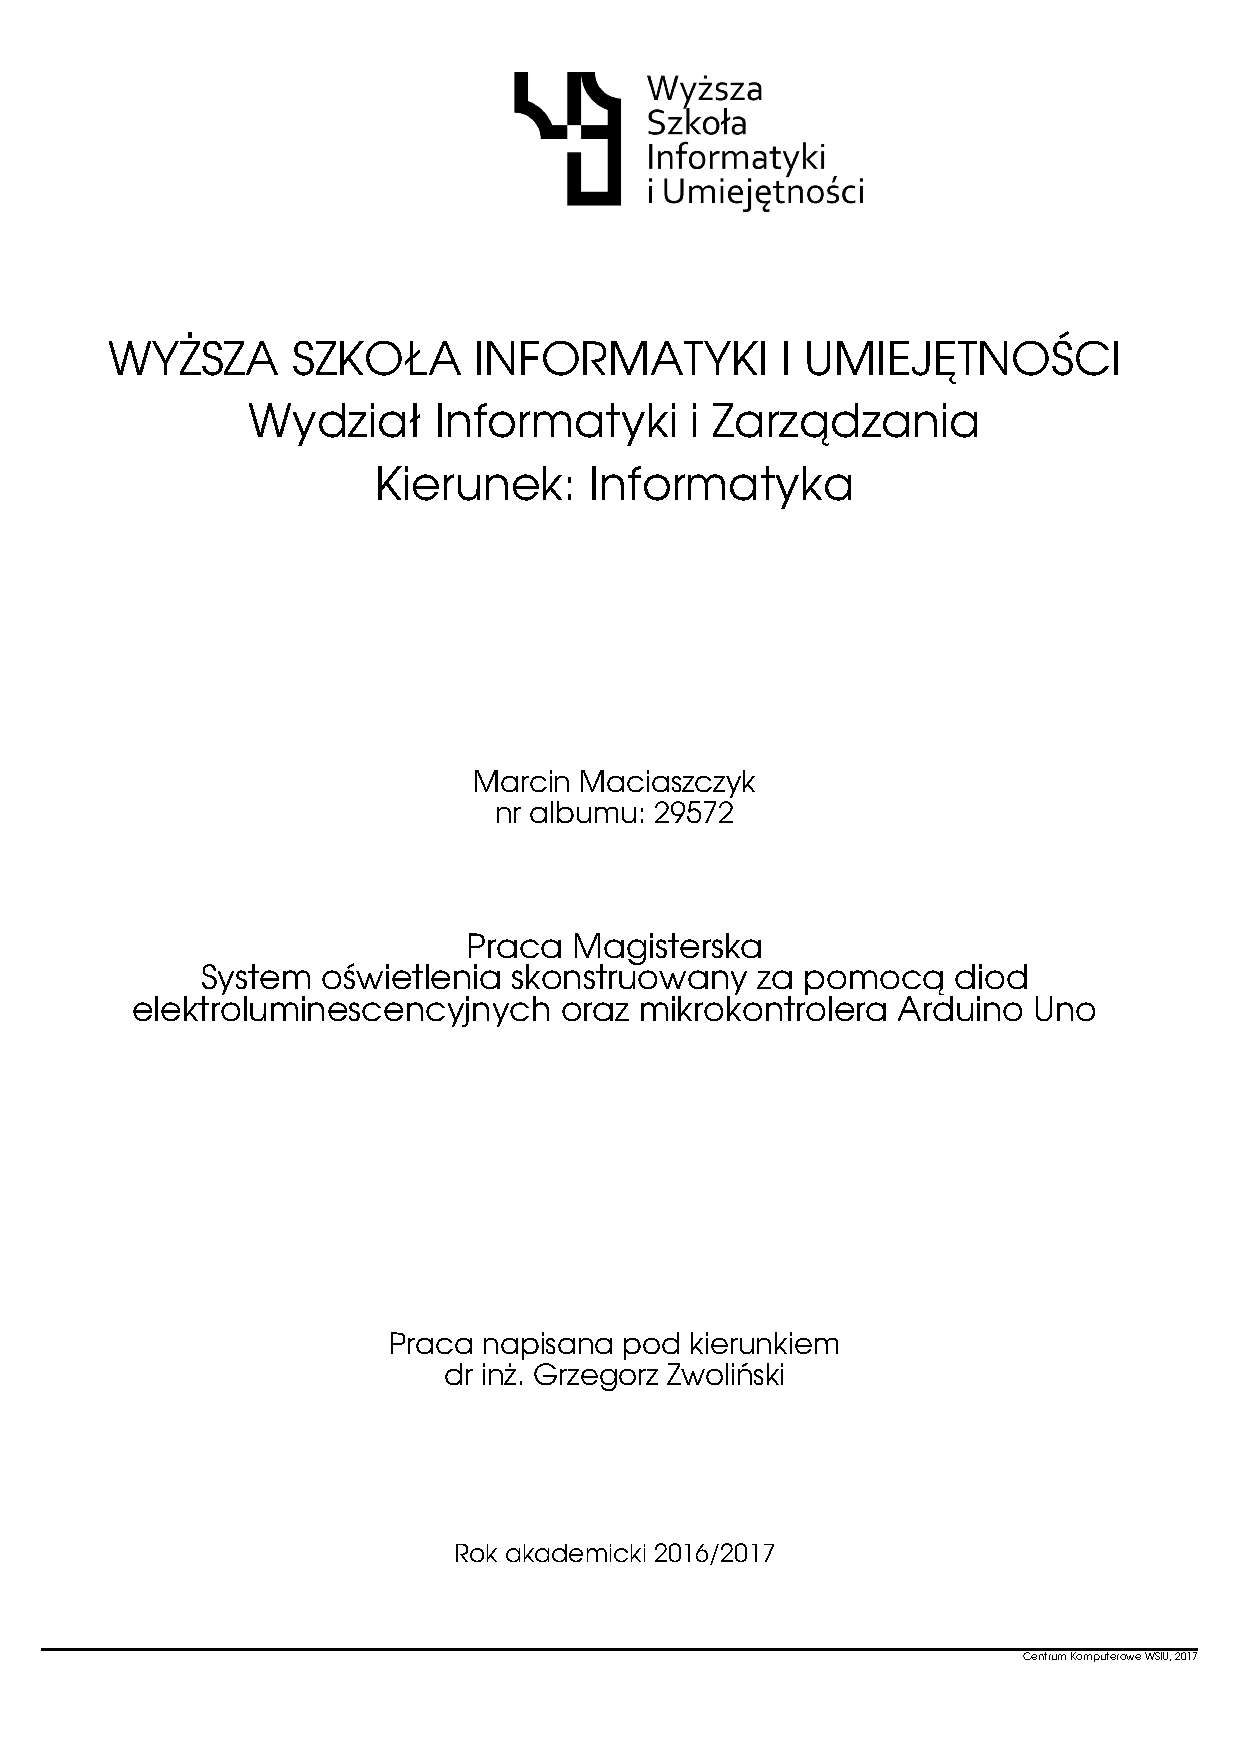
\includepdf[noautoscale=true, pages=-]{title-page.pdf}

\tableofcontents

\chapter{Wstęp}

\section{Uzasadnienie wyboru tematu}

Wraz z upływem czasu postęp technologiczny ma wpływ na życia co raz szerszej rzeszy ludzi na całym świecie. Niezliczone ilości urządzeń zagościły na stałe w domach i mało kto wyobraża sobie bez nich swoje życie. Zaczynając od artykułów gospodarstwa domowego, a kończąc na elektronice użytkowej do której zaliczają się komputery, telewizory czy też smartfony\footnote{~Przenośne urządzenia łączące w sobie zalety telefonów komórkowych oraz przenośnych komputerów (z ang. smartphone).}. Wszystkie te urządzenia mają na celu ułatwianie życia swoim użytkownikom.

W parze z licznymi zaletami urządzeń elektronicznych idą jednak pewne wady. Jedną z istotniejszych jest wpływ czasu spędzanego przed różnego rodzaju wyświetlaczami na zdrowie. Badania przeprowadzone na bazie danych Nielsen Audience Measurement pokazują, że przeciętny Polak spędza dziennie średnio 4,5 godziny przed ekranem telewizora\footnote{~Badania zostały przeprowadzone z uwzględnienem osób powyżej 4 roku życia w okresie od stycznia do czerwca 2015 roku \cite{czasprzedtv}.}. Nie oznacza to jednak, że przez cały ten czas ogląda on telewizję. Oglądanie filmów z dysku komputera, za pomocą serwisów VOD\footnote{~Wideo na życzenie (z ang. video on demand).} czy granie na konsoli także są wliczone w ten czas. Gdyby jednak dodać do tego czas spędzony przed ekranem smartfona czy też komputera wynik byłby zapewne dwukrotnie większy.

% TODO wsparcie co najmniej dwoma źródłami i coś o oglądaniu w ciemności
Pogorszenie wzroku czy też wysychanie gałki ocznej są wymieniane jako naj\-częstsze skutki zbyt dużej ilości czasu spędzanego przed ekranem. Poza próbą jego ograniczenia, jedną z częstszych porad jest próba zmniejszenia kontrastu pomiędzy ekranem a jego otoczeniem.

Do celów niniejszej pracy należy złożenie i oprogramowanie systemu oświetlenia, który ma rozszerzać obraz widziany na ekranie na jego otoczenie. Poza zmniejszeniem kontrastu, a więc aspektem zdrowotnym, system ma także na celu zwiększyć wrażenia wizualne dostarczane przez oglądany obraz.

% TODO krótkie wyjaśnienie podstawowych pojęć i diagram/zdjęcia
System oświetlenia składa się z taśmy diod elektroluminescencyjnych\footnote{~LED (z ang. light-emitting diode).} pod\-łączonych do mikrokontrolera Arduino Uno, który z kolei ma współpracować z komputerem z zainstalowanym systemem operacyjnym macOS. Oprogramowanie mikrokontrolera, którego zadaniem jest sterowanie diodami zostało przygotowane w języku Arduino, natomiast aplikacja kontrolująca cały system przeznaczona na komputer z systemem macOS została napisana w języku Swift. Wybór języków jest ściśle związany z koniecznością uzyskania jak najlepszej wydajności oraz użyciem najnowszych technologii.

Podobne systemy oświetlenia dostępne są już od pewnego czasu na rynku, jednak to właśnie nowoczesne technologie, prostota wykonania i niskie koszta powinny uczynić z Ligtning, bo taką nazwę otrzymał projekt, pełnowartościowego konkurenta.

\section{Problematyka i zakres pracy}

% TODO problematyka i zakres pracy

\section{Cele pracy}

% TODO cele pracy

\section{Metoda badawcza}

% TODO metoda badawcza

\section{Przegląd literatury w dziedzinie}

% TODO przegląd literatury w dziedzinie

\section{Układ pracy}

% TODO układ pracy

\chapter[Zagadnienia teoretyczne]{Zagadnienia teoretyczne}

% TODO zagadnienia teoretyczne

\chapter[Analiza istniejących rozwiązań]{Analiza istniejących rozwiązań}

\section{Kryteria analizy}

% TODO kryteria analizy

\section{Porównanie istniejących rozwiązań}

% TODO porównanie istniejących rozwiązań

\chapter{System oświetlenia Lightning}

\section{Analiza wymagań}

\subsection{Wymagania funkcjonalne}

W celu stworzenia jak najatrakcyjniejszego system oświetlenia podczas projektowania Lightning przyjęto poniższe wymagania funkcjonalne:

\begin{itemize}
\item System musi udostępniać tryb przechwytywania rozszerzający obraz wyświetlany na ekranie na jego otoczenie za pomocą diod elektroluminescencyjnych.
\item System musi posiadać tryb animacji. Powinien być on łatwy do rozszerzenia o kolejne animacje.
\item System musi być konfigurowalny z poziomu aplikacji sterującej. Konfiguracji podlegać musi co najmniej liczba i rozmieszczenie diod za ekranem, a także wykorzystywany port szeregowy.
\item Projekt musi być odpowiednio udokumentowany. Dokumentacja powinna ułatwiać szybkie skonfigurowanie oraz uruchomienie systemu.
\end{itemize}

\subsection{Wymagania niefunkcjonalne}

Do wymagań niefunkcjonalnych postawionych przed projektowanym systemem należą:

\begin{itemize}
\item System musi działać płynnie, a więc liczba osiąganych klatek na sekundę powinna być jak największa nawet przy dużych rozdzielczościach przechwytywanego ekranu.
\item Korzystanie z aplikacji sterującej powinno być jak najbardziej intuicyjne, a użytkownik powinien mieć dostęp do wskazówek dotyczących jej interfejsu.
\item Oprogramowanie mikrokontrolera powinno oferować jak najprostszy interfejs i zawierać jak najmniej logiki sterującej.
\item Pamięć na obu urządzeniach sterujących powinna być odpowiednio zarządzana, niedopuszczalne są wycieki pamięci czy też zapętlenia programu.
\end{itemize}

\section{Komponenty systemu}

Do konstrukcji systemu wykorzystane zostały następujące komponenty:

\begin{itemize}
	\item Cyfrowo adresowany łańcuch składający się z 25 diod elektroluminescencyjnych o średnicy 12 mm ze sterownikiem WS2801. Dostępny w sklepie internetowym Botland w cenie 195 zł \cite{diody}.
	\item Stabilizowany zasilacz sieciowy o napięciu wyjściowym 5 V. Dostępny w sklepie internetowym Botland w cenie 19,90 zł \cite{zasilacz}.
	\item Wtyk ze złączem pozawalającym połączyć łańcuch z zasilaczem. Dostępny w sklepie Botland w cenie 1,90 zł \cite{wtyk}.
	\item Mikrokontroler Arduino Uno w wersji 3. Dostępny w sklepie Botland w cenie 95 zł \cite{arduino}.
	\item Przewód USB. Dostępny w sklepie Botland w cenie 4,90 zł \cite{usb}.
\end{itemize}

Łańcuch z diodami został podłączony od jednej strony za pomocą wymienionego wcześniej wtyku z zasilaczem, z drugiej strony natomiast z mikrokontrolerem. Ten z kolei komunikuje się z komputerem z systemem macOS za pomocą przewodu USB. Dokładny schemat połączenia komponentów przedstawia rysunek \ref{schemat}.
	
\begin{figure}[h]
\centering
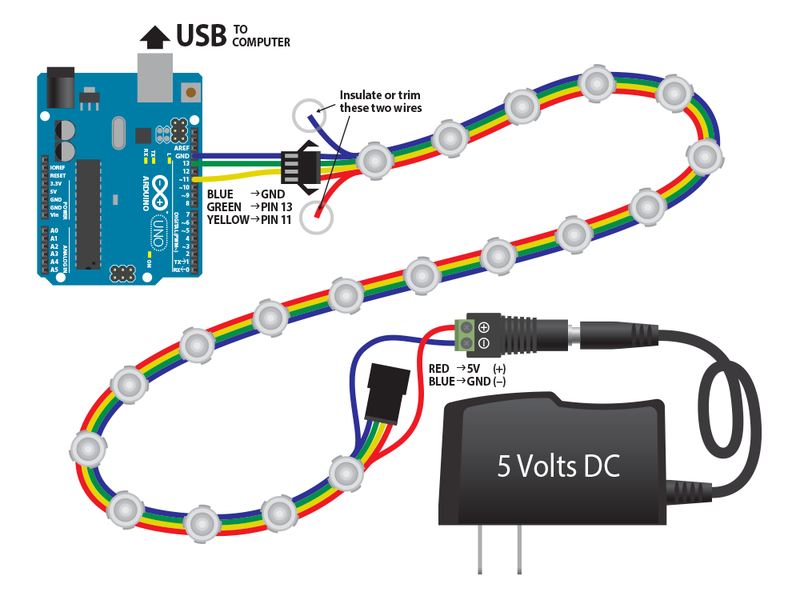
\includegraphics[width=\textwidth]{../resources/wiring.png}
\caption[Schemat podłączenia komponentów systemu]{Schemat podłączenia komponentów systemu \cite{schemat}}
\label{schemat}
\end{figure}
		
Koszt związany ze skompletowaniem wszystkich komponentów wyniósł łącznie 316,70 zł. Cena ta mogłaby ulec znacznemu zmniejszeniu w przypadku użycia kompatybilnych zamienników dla najdroższych elementów, czyli dla łańcucha diod czy też Arduino Uno w najnowszej wersji.

% TODO opis oraz zdjęcie mocowania diod

\section{Moduły oprogramowania}

\subsection{Oprogramowanie mikrokontrolera}

Głównym celem oprogramowania przeznaczonego na mikrokontroler jest zarządza\-nie diodami. Dzieje się to w oparciu o polecenia otrzymywane portem szeregowym od komputera, który steruje całym systemem. W związku z charakterem swojego zadania oprogramowanie musi działać jak najszybciej oraz posiadać jak najmniej logiki sterującej. Kontrola diod ogranicza się do przesyłania pakietów danych otrzymywanych z komputera na odpowiednie wyjścia do których diody są podłączone do mikrokontrolera. 

Moduł ten został napisany w natywnym języku Arduino, który udostępnia wszystkie podstawowe funkcje umożliwiające stworzenie oprogramowania spełniającego postawione przed nim wymagania.

\subsection{Aplikacja przeznaczona na komputer}

W przeciwieństwie do swojego poprzednika moduł przeznaczony na komputer ma za zadanie sterowanie całym systemem. Odpowiada on bezpośrednio na żądania użytkownika wydawane za pomocą stworzonego interfejsu graficznego i komunikuje się z oprogramowaniem mikrokontrolera w celu przekazania instrukcji zapalenia pewnej konfiguracji diod. Komunikacja odbywa się nieprzerwanie, jednokierunkowo, a każdy pakiet jest poprzedzony nagłówkiem składającym się z 11 bajtów.

Aplikacja ta może działać w dwóch trybach:

\begin{itemize}
	\item Tryb przechwytywania w którym przechwytywany jest obraz wybranego wyświetlacza, a każda dioda świeci się w kolorze odpowiadającego jej koloru ekranu. W trybie tym użytkownik powinien mieć kontrolę nad jasnością diod a także możliwość wygładzania przejść aby uniknąć szybkich zmian kolorów.
	\item Tryb animacji w którym za pomocą diod system wyświetla przygotowane wcześniej animacje. Animacje zapisane są jako klasy w języku Swift. Użytkownik poza wyborem animacji ma wpływ na użyte w niej kolory oraz prędkość animacji.
\end{itemize}

Ponadto aplikacja posiada możliwość konfiguracji liczby i rozmieszczenia diod, a także wykorzystywanego portu szeregowego.
Aplikacja została napisana w języku Swift, który jest przeznaczony dla komputerów z systemem macOS. Umożliwia on szybkie projektowanie interfejsów graficznych zgodnych z wyglądem systemu oraz przede wszystkim udostępnia on wszystkie podstawowe funkcje obiektowego języka programowania co jest istotne podczas projektowania aplikacji, której logika nie jest już tak prosta jak w przypadku oprogramowania mikrokontrolera.

\section{Projekt}

\subsection{System kontroli wersji}

Podczas pracy nad projektami programistycznymi często wymagana jest współpraca kilku programistów, cofanie pomyłkowo wprowadzonych zmian czy też dziennik zadań do wykonania. Wspomniane funkcjonalności udostępniają systemy kontroli wersji. Do najpopularniejszych należy Git, którego funkcjonalność darmowo udostępnia serwis   GitHub, gdzie z kolei znajduje się repozytorium projektu \cite{github}.

\begin{figure}[h]
\centering
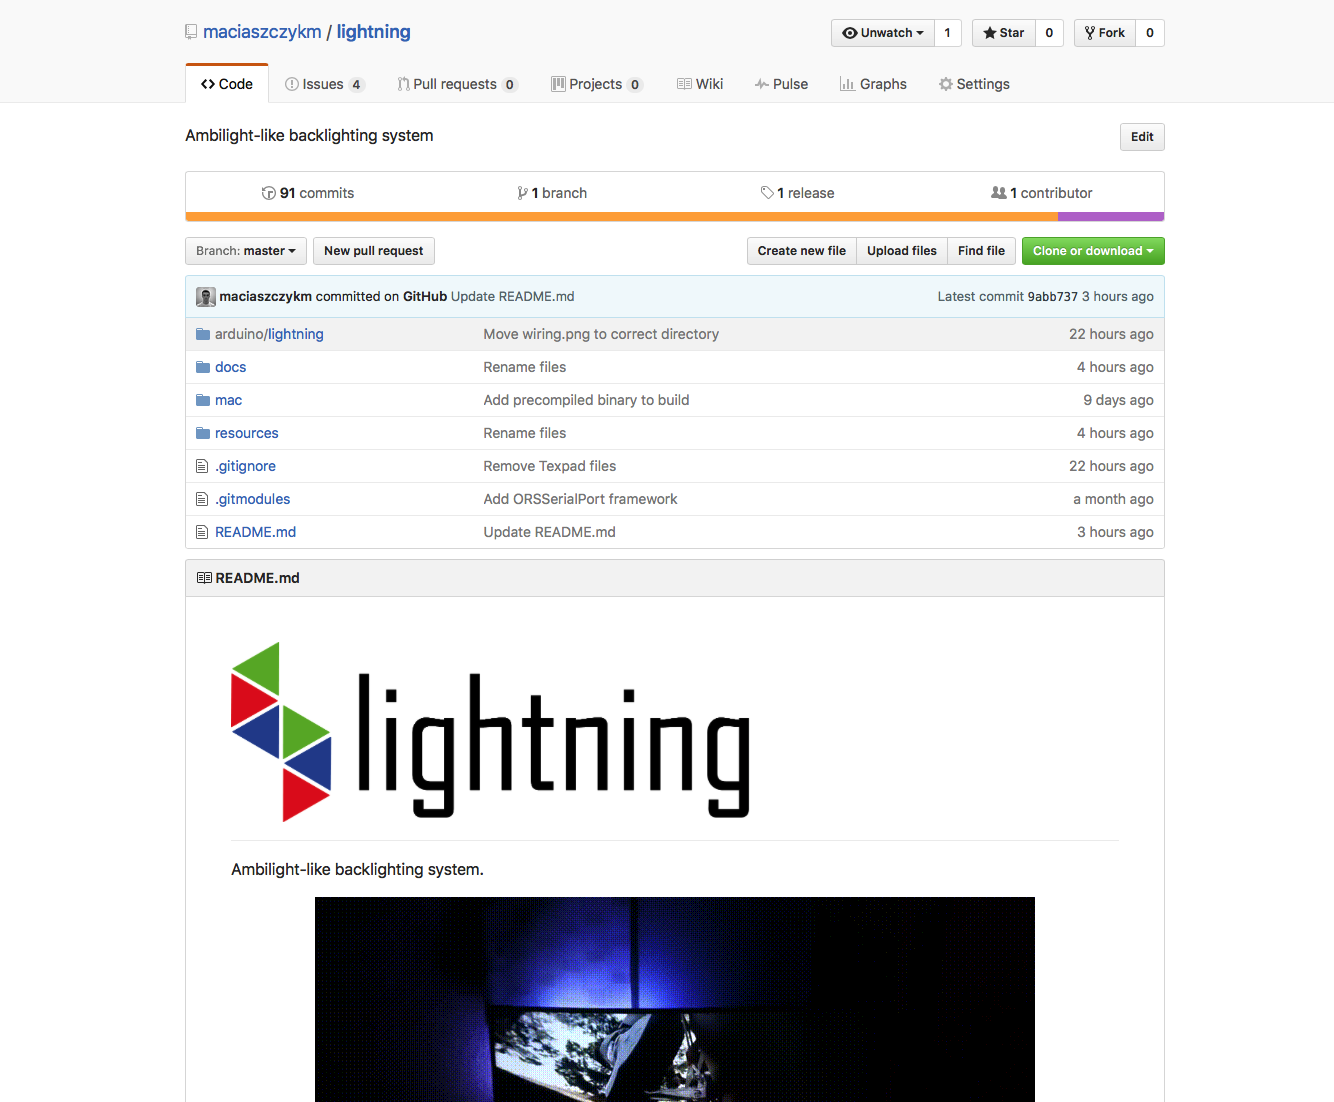
\includegraphics[width=\textwidth]{../resources/github.png}
\caption{Zrzut ekranu z repozytorium projektu}
\label{schemat}
\end{figure}

\subsection{Wykorzystane technologie}

Oprogramowanie mikrokontrolera zostało napisane w języku Arduino i to właśnie na tę platformę jest przeznaczone. Do jego napisania użyta została jedynie wbudowana biblioteka do obsługi portu szeregowego. Wykorzystano środowisko programistyczne Arduino \cite{arduinoide}.

Aplikacja sterująca została napisana w języku Swift, do stworzenia interfejsu graficznego wykorzystano framework\footnote{~Szkielet budowy aplikacji. Definiuje strukturę aplikacji oraz jej ogólny mechanizm działania, dostarcza zestaw komponentów i bibliotek ogólnego przeznaczenia do wykonywania określonych zadań.} Cocoa. Ponadto wykorzystano bibliotekę\\ORSSerialPort ułatwiającą komunikację poprzez port szeregowy \cite{orsserialport}. Wykorzystano środowisko programistyczne Xcode \cite{xcode}.

\subsection{Diagram klas}

% TODO diagram klas

\subsection{Wzorce projektowe}

% TODO wzorce projektowe

\subsection{Interfejs użytkownika}

\begin{figure}[h]
\centering

\includegraphics[width=\textwidth]{../resources/logo.png}
\caption{Logo projektu}
\end{figure}

Interfejs, w tym przypadku graficzny, należy do elementów na które użytkownicy zwracają uwagę na samym początku, dlatego też powinien być on zaprojektowany z pomysłem i umożliwiać jak najprostsze poruszanie się po aplikacji.
Aplikacja posiada dwa tryby działania oraz tryb konfiguracji, dlatego też logiczny jest podział na trzy widoki przedstawione poniżej:

% TODO interfejs użytkownika

\begin{itemize}
	\item 
\end{itemize}

\begin{figure}[h]
\centering
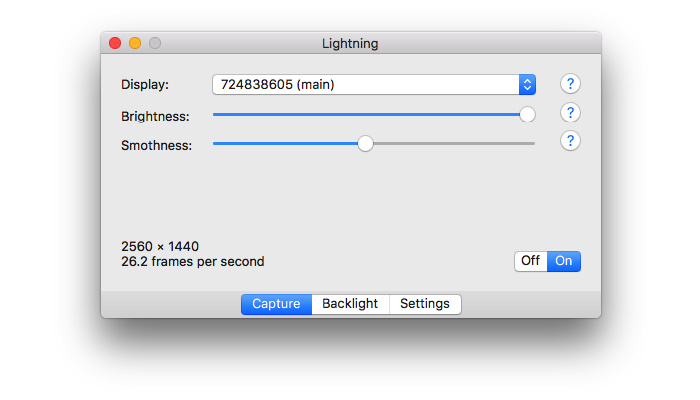
\includegraphics[width=\textwidth]{../resources/capture.png}
\caption{Widok trybu przechwytywania}
\end{figure}

\begin{figure}[h]
\centering
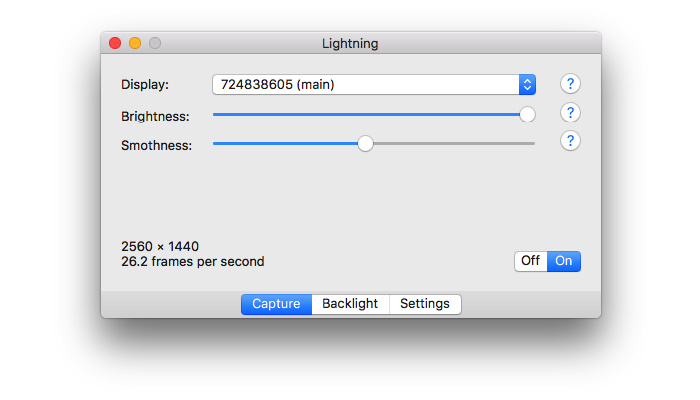
\includegraphics[width=\textwidth]{../resources/capture.png}
\caption{Widok trybu animacji}
\end{figure}

\begin{figure}[h]
\centering
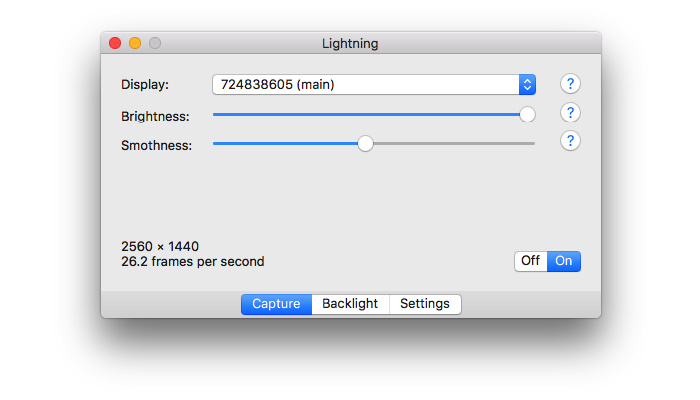
\includegraphics[width=\textwidth]{../resources/capture.png}
\caption{Widok konfiguracji}
\end{figure}

\section{Implementacja}

% TODO implementacja

\section{Podręcznik użytkownika}

% TODO podręcznik użytkownika

\section{Przykładowa implementacja animacji}

% TODO przykładowa implementacja animacji

\section{Analiza projektu}

% TODO analiza projektu

\section{Perspektywy rozwoju projektu}

% TODO perspektywy rozwoju projektu

\chapter{Podsumowanie}

\section{Dyskusja wyników}

% TODO dyskusja wyników

\section{Perspektywy rozwoju pracy}

% TODO perspektywy rozwoju pracy

\addcontentsline{toc}{chapter}{Bibliografia}
\begin{thebibliography}{99}
\bibitem{czasprzedtv} {\tt http://www.wirtualnemedia.pl/artykul/coraz-dluzej-ogladamy\-telewizje-najwiecej-czasu-przed-szklanym-ekranem-spedzaja\--seniorzy-raport}.\\Data dostępu -- 15.01.2017.
\bibitem{diody} {\tt https://botland.com.pl/lancuchy-i-matryce-led/2443-lacuch\-led-rgb-12-mm-ws2801-cyfrowy-adresowany-25-szt.html}.\\Data dostępu -- 17.01.2017.
\bibitem{zasilacz} {\tt https://botland.com.pl/zasilacze-sieciowe-5-v/1364-zasilacz\-impulsowy-5v-25a-wtyk-dc-55-21-mm.html}.\\Data dostępu -- 17.01.2017.
\bibitem{wtyk} {\tt https://botland.com.pl/szybkozlacza/1590-wtyk-dc-55-x-21\-mm-z-szybkozlaczem.html}.\\Data dostępu -- 17.01.2017.
\bibitem{arduino} {\tt https://botland.com.pl/arduino-moduly-glowne/1060-arduino\-uno-r3.html}.\\Data dostępu -- 17.01.2017.
\bibitem{usb} {\tt https://botland.com.pl/przewody-usb-a-b-20/5313-przewod\-usb-a-b-tracer-18m.html}.\\Data dostępu -- 17.01.2017.
\bibitem{schemat} {\tt https://cdn-learn.adafruit.com/assets/assets/000/001/484/\-medium800/led\_pixels\_wiring-diagram.png?1396773276}.\\Data dostępu -- 17.01.2017.
\bibitem{github} {\tt https://github.com/maciaszczykm/lightning}.\\Data dostępu -- 17.01.2017.
\bibitem{arduinoide} {\tt https://www.arduino.cc/en/main/software}.\\Data dostępu -- 18.01.2017.
\bibitem{orsserialport} {\tt https://github.com/armadsen/ORSSerialPort}.\\Data dostępu -- 18.01.2017.
\bibitem{xcode} {\tt https://developer.apple.com/xcode/}.\\Data dostępu -- 18.01.2017.
\end{thebibliography}

\addcontentsline{toc}{chapter}{Spis rysunków} 
\listoffigures

\addcontentsline{toc}{chapter}{Spis tabel} 
\listoftables

\addcontentsline{toc}{chapter}{Spis listingów} 
\lstlistoflistings

\end{document}